\documentclass[conference]{IEEEtran}
%\IEEEoverridecommandlockouts
% The preceding line is only needed to identify funding in the first footnote. If that is unneeded, please comment it out.
%Template version as of 6/27/2024
\usepackage{caption}
\usepackage{subcaption}
\usepackage[T1]{fontenc}


\usepackage{cite}
\usepackage{amsmath,amssymb,amsfonts}
\usepackage{amsthm}
\usepackage{algorithmic}
\usepackage{graphicx}
\usepackage{textcomp}
\usepackage{xcolor}
\usepackage{hyperref}

\newtheorem{theorem}{Theorem}
\newtheorem{assumption}{Assumption}
\newtheorem{lemma}{Lemma}
\newtheorem{statement}{Statement}
\newtheorem{proposition}{Proposition}
\newtheorem{corollary}{Corollary}


\def\BibTeX{{\rm B\kern-.05em{\sc i\kern-.025em b}\kern-.08em
    T\kern-.1667em\lower.7ex\hbox{E}\kern-.125emX}}
\begin{document}

\title{ConvNets Landscape Convergence: Hessian-Based Analysis of Matricized Networks}
% 1. Hessian Decomposition for Matricized Networks and Convolutions
% 2. Hessian Matrix of Matricized Networks: Loss Landscape of Convolutions
% 3. Hessian-Based Analysis of Matricized ConvNets
% 4. Hessian Norm in Matricized ConvNets: Parameters & Performance
% ConvNets Landscape Convergence: Hessian-Based Analysis of Matricized Networks

%\author{
%\IEEEauthorblockN{1\textsuperscript{st} Vladislav Meshkov}
%\IEEEauthorblockA{
%\textit{Moscow Institute of Physics and Technology}\\
%Moscow, Russia \\
%meshkov.vs@phystech.su}
%\and
%\IEEEauthorblockN{2\textsuperscript{nd} Nikita Kiselev}
%\IEEEauthorblockA{
%\textit{Moscow Institute of Physics and Technology}\\
%Moscow, Russia \\
%kiselev.ns@phystech.su}
%\and
%\IEEEauthorblockN{3\textsuperscript{rd} Andrey Grabovoy}
%\IEEEauthorblockA{
%\textit{Moscow Institute of Physics and Technology}\\
%Moscow, Russia \\
    %grabovoy.av@phystech.su}}

% latin bold lower
\newcommand{\ba}{\mathbf{a}} 
\newcommand{\bc}{\mathbf{c}} 
\newcommand{\be}{\mathbf{e}} 
\newcommand{\bh}{\mathbf{h}} 
\newcommand{\bp}{\mathbf{p}} 
\newcommand{\bt}{\mathbf{t}} 
\newcommand{\bs}{\mathbf{s}} 
\newcommand{\bu}{\mathbf{u}} 
\newcommand{\bv}{\mathbf{v}} 
\newcommand{\bw}{\mathbf{w}} 
\newcommand{\bx}{\mathbf{x}} 
\newcommand{\by}{\mathbf{y}} 
\newcommand{\bz}{\mathbf{z}} 
\newcommand{\bm}{\mathbf{m}} 

% latin bold upper
\newcommand{\bA}{\mathbf{A}} 
\newcommand{\bB}{\mathbf{B}} 
\newcommand{\bC}{\mathbf{C}} 
\newcommand{\bG}{\mathbf{G}}
\newcommand{\bF}{\mathbf{F}}
\newcommand{\bI}{\mathbf{I}} 
\newcommand{\bJ}{\mathbf{J}} 
\newcommand{\bL}{\mathbf{L}} 
\newcommand{\bM}{\mathbf{M}} 
\newcommand{\bH}{\mathbf{H}}
\newcommand{\bP}{\mathbf{P}}
\newcommand{\bQ}{\mathbf{Q}} 
\newcommand{\bR}{\mathbf{R}} 
\newcommand{\bT}{\mathbf{T}} 
\newcommand{\bU}{\mathbf{U}} 
\newcommand{\bV}{\mathbf{V}} 
\newcommand{\bW}{\mathbf{W}} 
\newcommand{\bX}{\mathbf{X}} 
\newcommand{\bY}{\mathbf{Y}} 
\newcommand{\bZ}{\mathbf{Z}} 

% latin cal upper
\newcommand{\cF}{\mathcal{F}} 
\newcommand{\cG}{\mathcal{G}} 
\newcommand{\cI}{\mathcal{I}} 
\newcommand{\cL}{\mathcal{L}} 
\newcommand{\cM}{\mathcal{M}} 
\newcommand{\cN}{\mathcal{N}} 
\newcommand{\cS}{\mathcal{S}} 
\newcommand{\cT}{\mathcal{T}} 
\newcommand{\cW}{\mathcal{W}} 
\newcommand{\cX}{\mathcal{X}} 
\newcommand{\cY}{\mathcal{Y}} 
\newcommand{\cZ}{\mathcal{Z}} 

% latin bb upper
\newcommand{\bbE}{\mathbb{E}} 
\newcommand{\bbI}{\mathbb{I}} 
\newcommand{\bbP}{\mathbb{P}} 
\newcommand{\bbR}{\mathbb{R}}
\newcommand{\bbX}{\mathbb{X}} 
\newcommand{\bbY}{\mathbb{Y}}
\newcommand{\bbW}{\mathbb{W}} 

% greek bold lower
\newcommand{\bLambda}{\boldsymbol{\Lambda}}

\newcommand{\bepsilon}{\boldsymbol{\epsilon}} 
\newcommand{\btheta}{\boldsymbol{\theta}} 
\newcommand{\blambda}{\boldsymbol{\lambda}} 
\newcommand{\bpi}{\boldsymbol{\pi}} 
\newcommand{\bmu}{\boldsymbol{\mu}} 
\newcommand{\bsigma}{\boldsymbol{\sigma}} 
\newcommand{\bphi}{\boldsymbol{\phi}} 

% greek bold upper
\newcommand{\bSigma}{\boldsymbol{\Sigma}} 

% transpose
\newcommand{\T}{^{\text{\tiny\sffamily\upshape\mdseries T}}}

\newcommand{\norm}[1]{\left\|#1\right\|}

%\author{
%\IEEEauthorblockN{\textbf{Anonymous authors}\\Paper under double-blind review}
%}

\maketitle
\newcommand{\f}[1]{f_{\btheta}(#1)}
\begin{abstract}
The Hessian of a neural network is an important aspect for understanding the loss landscape and the characteristic of network architecture. The Hessian matrix captures important information about the curvature, sensitivity, and local behavior of the loss function. Our work proposes a method that enhances the understanding of the local behavior of the loss function and can be used to analyze the behavior of neural networks and also for interpreting the parameters in these networks. In this paper, we consider an approach to investigate the properties of the deep neural network, using the Hessian. We propose a method for estimating the Hessian matrix norm for a specific type of neural networks like convolutional. We have obtained the results for both 1D and 2D convolutions, as well as for the fully connected head in these networks. Our empirical analysis supports these findings, demonstrating convergence in the loss function landscape. We have evaluated the Hessian norm for neural networks represented as a product of matrices and considered how this estimate affects the landscape of the loss function.
\end{abstract}

%%%%%%%%%%%%%%%%%%%%%%%%%%%%%%
% TODO: mb I need
%%%%%%%%%%%%%%%%%%%%%%%%%%%%%%
%\begin{IEEEkeywords}
%first, second, third.
%\end{IEEEkeywords}

\section{Introduction}\label{sec:intro}

The loss landscape is important for understanding the nature of deep network parameters \cite{shinshilla, relevance, ordering}. Often it helps to understand differences between architectures \cite{loss-landscape, skip-conn-landscape}, significance of activation \cite{Bosman_2023} and local and global minima properties \cite{BOSMAN2020113, neyshabur2018the, improved_analysis_trianing}. \\
Many studies have investigated the loss function landscape for modern architectures, for instance, \cite{lee2024visualizinglosslandscapeselfsupervised} investigates the self-supervised ViT through the lens of the loss landscape, \cite{chen2022visiontransformersoutperformresnets} investigates ViTs and MLP-Mixers from the lens of loss geometry, intending to improve the models’ data efficiency at training and generalization at inference. Paper \cite{elhamod2023neurovisualizerautoencoderbasedlosslandscape} presents a landscape visualization
method that provides useful insights about neural network loss landscapes. The authors of \cite{bain2021visualizinglosslandscapewinning} reduce the time required to compute such loss landscapes. Studies \cite{Exp_explor_loss_surface, im2017empiricalanalysisoptimizationdeep} conduct experimental exploration on the loss surface of the deep neural network, including trajectories of various adaptive optimization algorithms. Numerous works have examined the spectrum of the Hessian matrix \cite{investigation_neural_net_eigen, full_spec_hess, liao2021hessianeigenspectrarealisticnonlinear} or established upper bounds on the rank of a matrix. For instance, \cite{singh2023hessianperspectivenatureconvolutional} estimated the ranks of Hessian blocks through their decomposition.  \\
In this work, we derive theoretical estimates for the spectral norm of the Hessian. We demonstrate that the spectral norm of the Hessian provides an upper bound on the difference between the mean values of the loss function when incorporating an additional object into the sample. This leads to further applications related to sample size determination \cite{sample-size-det} and offers insights into the manner in which parameters can influence the Hessian matrix.
We propose a theoretical analysis for decomposing the Hessian into linear components and provide specific applications to convolutional networks.
First, we investigate the behavior of the loss function in the vicinity of the optimum. We examine how the loss landscape near the solution and the Hessian norm depend on the specific network architecture. \\
Another objective of this study is to understand how the norm of parameters, along with their quantity and spatial distribution within the neural network, influences the learning process \cite{azadbakht2022drasticallyreducingnumbertrainable, wu2019prodsumnetreducingmodelparameters, kahatapitiya2020exploitingredundancyconvolutionalfilters}, where the meaning of parameters and ways to reduce their number are described in detail.
Additionally, a crucial aspect of this work is the evaluation of the absolute difference between the average loss function values at successive steps, which is derived directly from our estimation of the Hessian norm.

Our contributions can be summarized as follows:
\begin{itemize}
    \item We present a method for the decomposition of the Hessian matrix into linear components and apply this approach to estimate the norm of the Hessian matrix.
    \item We illustrate the application of our results to convolutional architectures and provide insights into the relationship between parameters and their corresponding estimates.
    \item We demonstrate the validity of our theoretical results through experiments on image classification, using convolutional networks.
\end{itemize}


\section{Related Work}\label{sec:rw}

\textbf{Neural Network Loss Landscapes}.
The landscape of loss functions has been explored from various perspectives in the literature. For instance,\cite{DBLP:journals/corr/abs-1910-05929} show connections between a number of classes and directions of high positive curvature. Paper \cite{skip-conn-landscape} shown, that the loss landscape of the two-layer
ReLU network has good properties when the number of hidden nodes is large.
Work \cite{singh2024landscapinglinearmodeconnectivity} offers a model of how the loss landscape needs to behave topographically for LMC(linear mode connectivity). Work \cite{categ_plots} categorizes the loss
surfaces curves, plotted along Gaussian noise directions. The properties of neural networks and their Hessian spectra near the interpolation threshold are uncovered by \cite{singh2022phenomenologydoubledescentfinitewidth}.
Works \cite{lee2024visualizinglosslandscapeselfsupervised, chen2022visiontransformersoutperformresnets} explore the ViT architecture using the local landscape of the loss function.
However, these works are based on specific architectures. % TODO: mb more

\textbf{Analyzing the Hessian Matrix}.
The decomposition of the Hessian matrix into its components is a key tool for studying its properties.
The decoupling conjecture, which decomposes the layer-wise Hessians of a network as the Kronecker product of two smaller matrices, is proposed by \cite{DissectingHessian}. In \cite{skorski2019chainruleshessianhigher} we can see Hessian chain rule and useful tensor calculations associated with it. However, these studies have not been extended to analyze the loss function landscape through the use of the Hessian matrix norm.

\textbf{Hessian eigenvalues and eigenspectra}.
The spectrum of the Hessian matrix is crucial for understanding the structure of the loss function landscape.
Authors of the work \cite{investigation_neural_net_eigen} develop a tool to study
the evolution of the entire Hessian spectrum
throughout the optimization process. The authors of \cite{papyan2019spectrumdeepnethessiansscale} efficiently approximate the spectrum of the Hessian of neural networks, through decomposing the Hessian into different components. At work \cite{sagun2017eigenvalueshessiandeeplearning} we can see empirical evidence, that eigenvalue distribution can be composed of two parts: which is concentrated around zero, and which are scattered away from zero. Authors of \cite{papyan2020tracesclasscrossclassstructurepervade} identify and discuss an important formal class/cross-class structure and show how it lies at the origin of the many features observed in deep networks spectra.
The existence of outliers in the spectrum of the Hessian is addressed by \cite{papyan2019measurementsthreelevelhierarchicalstructure}, who attempt to provide an explanation.
The authors of \cite{liao2021hessianeigenspectrarealisticnonlinear} make a characterization of the
Hessian eigenspectra for a broad family of nonlinear models.
Paper \cite{azadbakht2022drasticallyreducingnumbertrainable} develops a
tool to study the evolution of the entire Hessian spectrum throughout the optimization process.
The authors of \cite{kiselev2024unravelinghessiankeysmooth} have covered the topic most accurately, the paper proposes a method for investigating the spectrum when changing the sample size, but they are limited to only the fully connected neural network.



\section{Preliminaries}\label{sec:prelim}

\subsection{General notation}
In this section, we introduce the general notation used in the rest of the paper and the basic assumptions. Similar to \cite{Matrixdifferential} we consider matrix derivatives, using vectorize row-wise ($vec_r$). For given $\bX \in \bbR^{m \times n}, \bY \in \bbR^{p \times q}$ we define:
\begin{align*}
\frac{\partial \bX}{\partial \bY} := \frac{\partial vec_r\bX}{\partial (vec_r\bY)\T}.
\end{align*}
For higher tensor dimension we define it in the same way. Having $K$-label classification problem, we consider a probability $p(\by | \bx)$, that maps unobserved $\bx \in \mathcal{X}$ to corresponding output $\by \in \mathcal{Y} = \bbR^K$~--- one-hot vectors, where $K$~--- number of classes. We have a neural network $f_{\btheta}$, parameterized by $\btheta \in \bbR^{p}$:
Let i.i.d. dataset of size m:
\[\mathfrak{D} = \{\bx_i, \by_i\}_{i=1,...,m}.\]
Our loss function is CE, let loss on $\bx_i$ and $\by_i$ be the:
\[ \ell_i(\btheta) := \ell(\f{\bx_i}, \by_i).\]
Empirical loss function for the first k elements:
\[\cL_k(\btheta) := \frac{1}{k}\sum\limits_{i=1}^k \ell_i(\btheta), \quad \cL(\btheta) := \cL_m(\btheta).\]
Our objective is empirical loss function on the whole sample
\[ \cL_m = \frac{1}{m}\sum\limits_{i=1}^m\ell_i(\btheta) \approx \bbE_{p(\bx, \by)}\ell(\f{\bx_i}, \by_i).\]
One of our goals will be to estimate this difference.
\[\cL_{k+1}(\btheta) - \cL_{k}(\btheta) = \frac{1}{k+1}\big(\ell_{k+1}(\btheta) - \cL_{k}(\btheta)\big).\]
We introduce several definitions related to derivatives.
Jacobian of the NN:
\[J(\btheta) := J_{\f{\bx}} = (\nabla_{\btheta}f_{\btheta}(\bx))\T.\]
The total Hessian is written as:
\[\bH^{(k)}(\btheta) := \nabla^2_{\btheta}\cL_k(\btheta) = \frac{1}{k}\sum\limits_{i=1}^k\nabla_{\btheta}^2\ell_i(\btheta).\]


\subsection{Assumptions} 
To compare losses and arrange them in one point it would be convenient to introduce the following assumption.
\begin{assumption}\label{assumpt}
    Let $\btheta^*$ be the local minimum of both $\cL_{k}(\btheta)$ and $\cL_{k+1}(\btheta)$.
    In particular, it means, that $\nabla_{\btheta}\cL_{k}(\btheta^*) = \nabla_{\btheta}\cL_{k+1}(\btheta^*) = 0$.
\end{assumption}
This assumption allows us to study the behavior of the landscape using only one point.

\subsection{Approximation and Decomposition} 
Using this assumption and second-order approximation, in the work \cite{kiselev2024unravelinghessiankeysmooth} it is shown, that to study local behavior one can use second-order Taylor approximation, from which we get
\begin{multline}\label{eq:diff}
\big|\cL_{k+1}(\btheta) - \cL_{k}(\btheta)\big| \approx \frac{1}{k+1}\big|\ell_{k+1}(\btheta^*) - \cL_k(\btheta^*)\big| + \\
 + \frac{1}{k+1}\norm{\btheta - \btheta^*}^2\norm{\bH_{k+1}(\btheta^*) - \frac{1}{k}\sum\limits_{i=1}^k\bH_i(\btheta^*)}.
\end{multline}


It is well known \cite{schraudolph2002}, that via chain rule, we can decompose out Hessian: 
Let $\bH$ be the Hessian of $\ell$ on object $\bx$, then

\begin{align*}
\bH = \bH_O + \bH_F = J(\btheta)\T\left[\nabla^2_{f_{\btheta}}\ell(\btheta)\right]J(\btheta) + \\
+ \sum\limits_{c = 1}^K\left[\nabla_{f_{\btheta}}\ell(\btheta)\right]_c\nabla^2_{\btheta}f^c_{\btheta}(\bx).
\end{align*}

As \cite{DBLP:journals/corr/SagunEGDB17, DBLP:journals/corr/abs-1910-05929} can use only $\bH_O$, because, at a point close to a local minimum, the average gradient is close to zero, then we can neglect the $\bH_F$ term. Based on this approximation we will consider the norm of $\bH_O$ term matrix.
So, in terms of the matrix norm 
\begin{equation}
    \norm{\bH} \approx \norm{J(\btheta)\T\left[ \nabla^2_{f_{\btheta}} \ell (\btheta)\right] J(\btheta)}.
\end{equation}


\subsection{Outer-product Hessian}
We adopt the term \guillemotleft outer-product\guillemotright \space Hessian for the $\bH_O$ term, as in \cite{singh2021analyticinsightsstructurerank}. As we will see later, it is in this form that it is most convenient to analyze the Hessian. In particular, we note that $\nabla_{\f{\btheta}}^2\ell(\btheta)$ depends only on loss function, for example: \\
for MSE loss: $\nabla_{\f{\btheta}}^2\ell(\btheta) = I$ \\
for CE(cross-entropy) loss: $\nabla_{\f{\btheta}}^2\ell(\btheta) = diag(\bp) - \bp\bp\T$, \\
where $p := \mathrm{SoftMax}(\bz).$
The choice of loss function is inconsequential, affecting only a multiplicative constant that does not influence the overall analysis. We estimate the norm of matrix products by considering the product of their individual norms, leading to a quadratic dependence of the Hessian norm on the Jacobian in approximate calculations. As noted in \cite{hayou2024a}, the Jacobian provides valuable structural insights into the network, which we examine further.

\section{matrix-product network representation}
Let $\f{\bx}$ be the composition of $L+1$ layers with ReLU activations
\[\f{\bx} = \bT^{(L+1)} \circ \sigma \circ \dots \circ \sigma \circ \bT^{(1)}(\bx).\]
$\bT^{(p+1)}$ ~--- linear operator (or its matrix), $\sigma$ ~--- ReLU activation, the intermediate results can be represented as
\begin{align*}
  \begin{cases}
    & \bz^{(p+1)} = \bT^{(p+1)}\bx^{(p)}, \\
    & \bx^{(p+1)} = \sigma(\bz^{(p+1)})
  \end{cases}
\end{align*}
with output logits $f_{\btheta}(\bx) = \bz := \bz^{(L+1)}$, and input $\bx^{(0)} := \bx$. \\
Let $\bLambda^{(p+1)} := diag(\bx^{(p+1)} > 0)$ be input-dependent matrix. \\
Then $\f{x}$ has the form of a product of matrices (m.b. input-dependent)
\begin{equation}\label{eq:net-repr}
\f{x} = \bT^{(L+1)}\bLambda^{(L)}\dots \bLambda^{(1)}\bT^{(1)}\bx. \\
\end{equation}
The vector of weights is also considered $\btheta = col(\bW^{(L+1)}, \dots, \bW^{(1)})$, where $\bT^{(p)}$ id differentiable and parameterized by part $\bW^{(p)}$. Then the derivative of a layer with respect to its parameters can be determined. \\
\[\bQ^{(p)} := \frac{\partial \bT^{(p)}}{\partial \bW^{(p)}},\]
\[\bQ:= diag({\bQ}^{(1)}, \dots, {\bQ}^{(L+1)})\]
Where $\bQ^{(p)}$ matrix gives a complete description of how the parameters are arranged in the p-th layer. \\
To simplify further formulas we define
\[ \bG^{(p)} := \bT^{(L+1)}\bLambda^{(L)} \dots \bT^{(p+1)}\bLambda^{(p)}; \bG^{(L+1)} := \bI \]
\[\bR^{(p)} := \bLambda^{(p)}\bT^{(p)} \dots \bLambda^{(1)}\bT^{(1)};\;\;p = \overline{1,L}; \; \bR^{(0)} := \bI.\]
Using notation, we can rewrite
\begin{align*}
& \bz = \bG^{(p)}\bz^{(p)},\; \bx^{(p)} = \bR^{(p)}\bx, \\
& \bz = \f{\bx} = \bG^{(p)}\bT^{(p)}\bR^{(p-1)}\bx.
\end{align*}
The stacked matrices $\bG^{(p)}$ and $\bR^{(p)}$ give us
\begin{align*}
\bF\T := 
    \begin{pmatrix}
        \bG^{(1)\T} \otimes \bR^{(0)}\bx \\
        \vdots \\
        \bG^{(k)\T} \otimes \bR^{(k-1)}\bx \\
        \vdots \\
        \bG^{(L+1)\T} \otimes \bR^{(L)}\bx
    \end{pmatrix}.
\end{align*}
The Hessian of a neural network by logits in case of CE loss function
\[ \bA := \nabla^2_{\bz} \ell = diag(\bp) - \bp\bp\T, \]
where $\bp := \mathrm{softmax}(\bz)$.


\subsection{Hessian Structure}
According to papers \cite{DissectingHessian, kiselev2024unravelinghessiankeysmooth, singh2023hessianperspectivenatureconvolutional} we can decompose outer-product Hessian into simpler components, more specifically, we need to decompose only the Jacobian.

We will consider the key Lemmas of this paper, which describe the decomposition of the Hessian into a product of 5 matrices and the use of this representation to estimate the norm, the proofs are given in the appendix ~\ref{app:lemma:hesstruct} and ~\ref{app:lemma:hessnorm}.

\begin{lemma}\label{lemma:hesstruct}
    Let our net $\f{\bx}$ can be represented as   \eqref{eq:net-repr}, then
    $\bH_O(\btheta) = \bQ\T\bF\T\bA\bF\bQ$.
\end{lemma}


\begin{lemma}\label{lemma:hessnorm} 
    Let the net $\f{\bx}$ can be represented as $\eqref{eq:net-repr}$  \\
    Let $\forall p: \;\; \norm{\bQ^{(p)}} \leqslant q,\; \; \norm{\bT^{(p)}}^2 \leqslant w_{\bT}^2.$ \\
    Then we have: \\
    $\norm{\bH_O} \leqslant \sqrt{2}q^2\norm{\bx}^2(L+1)w_{\bT}^{2L}.$
\end{lemma}

These lemmas are used to estimate the Hessian norms in special cases.

\section{convolutions}
\subsection{1D convolution}
In this section, for simplicity, we keep the notation $\bT^{(p)}$, but use it for 1D-convolutions, and we will explain how they are represented as linear operators.
It is well known that convolutional networks can often be represented by a linear convolutional neural network (LCN). This usually refers to the Toeplitz representation of CNNs. \cite{kohn2022geometrylinearconvolutionalnetworks, qin2023toeplitzneuralnetworksequence}.
In this paper we use the notation for Toeplitz matrices from \cite{singh2023hessianperspectivenatureconvolutional}.
Also in the paper the authors found a specific type of matrix $\bQ^{(p)}$, according to the structure of 1D Toeplitz matrix.
Our 1D convolutional network is $\f{\bx} = \bT^{(L+1)} * (\sigma(\dots (\sigma(\bT^{(1)} * \bx))\dots)$, where operation $*$ means convolution. \\
Let $C_p$ be the number of channels after the $p$-th layer, and $d_p$ be the size of sequence. There $\bx^{(p)} \in \bbR^{C_p \times d_p}$, $\bT^{(p)}$-1D convolution layer with kernel  $\bW^{(p)} \in \bbR^{C_{p-1} \times C_{p} \times k_{p}}$. 
To simplify further notations we can replace 
$\bx^{(p)}$ with $vec(\bx^{(p)}) \in \bbR^{(C_pd_p)}$. 
Now we have:
\[\bz^{(p+1)} = \bT^{(p+1)}\bx^{(p)}.\]
The main results for 1D convolutions, which uses Toeplitz matrices to calculate $\bT^{(p)}$ and $\bQ^{(p)}$ like in \cite{singh2023hessianperspectivenatureconvolutional} (out notation for the convolutions and Toeplitz matrices are identified for simplicity), and Lemmas ~\ref{lemma:hesstruct} and ~\ref{lemma:hessnorm}. For more details see the proof in the appendix: ~\ref{app:thm:1Dconv}.
\begin{theorem}\label{thm:1Dconv}
    Consider the net $\f{x} = C_{\bW^{(L+1)}} \circ \sigma \circ \dots \circ \sigma \circ C_{\bW^{(1)}}$, where $C_{\bW^{(i)}}$ - 1D convolution with kernel $\bW^{(i)}$, without padding and with stride=1. Let the following upper bounds be given:
     $C_l \leqslant C$,
     $k_i \leqslant k$,
     $d_i \leqslant d_1:=d$,
     $|\bW^{(p)}_{i,j,k}|^2 \leqslant w^2$. Then we can estimate outer-product hessian norm\\
    \[\norm{\bH_{O}} \leqslant \sqrt{2}\norm{x}^2d^2(L+1)(C^2w^2kd)^L.\]
\end{theorem}
As investigation, we apply this theorem to the difference of loss, same as \cite{kiselev2024unravelinghessiankeysmooth}.
\begin{corollary}
let $\btheta$ be in the $R$-vicinity of optima: \\ $\norm{\btheta - \btheta^*} \leqslant R$. Loss function is limited by some constant: $\exists \; W_l > 0: \; \forall i\; |\ell_i| \leqslant W_l$. Let all objects in the dataset are limited too: $\exists W_x\; \forall i \; \norm{x_i} \leqslant W_x$. Then, under the conditions of the theorem ~\ref{thm:1Dconv} and our assumptions, we have:
\begin{align*}
& \big|\cL_{k+1}(\btheta) - \cL_{k}(\btheta)\big| \leqslant \frac{2}{k+1}W_{\ell} +\\
& + \frac{2}{k+1}R^2\sqrt{2}d^2W_x^2(L+1)(C^2w^2kd)^L.
\end{align*}
\end{corollary}

As we can see, this estimate is extremely high compared to the actual norm. However, one can hypothesize that the dependence on the number of channels, the weight norms, and the sizes is indeed the same as presented above. We suppose that if the parameters for convolution are already sufficient for training, then increasing, for example, the size of the convolution kernel k will unjustifiably increase the estimate ,approximately by a factor of $(1 + \frac{\Delta k}{k})^L$, which can lead to a slowdown in the rate of convergence without significant improvements in quality.

\subsection{2D-convolution}\label{sec:2d-conv}
In this section we consider 2D convolutional networks. Again, for simplicity, we retain the $\bT^{(p)}$ notation for convolutional network layers, and we will explain why convolution can be considered a linear layer. $\bx \in \bbR^{m \times n \times C}$ - input image, which has (m, n) dimentions and C channels. \\
$\bx^{(l)} \in \bbR^{m_i \times n_i \times C_i}$ - input of $l+1$-th layer. 
$\bW^{(l)} \in \bbR^{C_{l-1} \times C_l \times k^1_l \times k^2_l}$ - convolution with kernel sizes $(k^1_l, k^2_l)$, input and output numbers of channels $C_{l-1}, C_l$ respectively. 
Similar to the section A, we use $vec(\bx) \in \bbR^{m_in_iC_i}$ instead of $\bx \in \bbR^{m_i \times n_i \times C_i}$.
The operation of convolution on the input tensor is examined, particularly in the case of a vectorized input. We can use the same Toeplitz framework as in \cite{toep_2dconv}, but it's easier for us to use a specific matrix $\bT^{(p)}$, a row of which consists of elements $\bW^{(p)}_{*, c_2, *, *}$ for the $c_2$-th channel. That is, each row of $\mathbf{T}^{(p)}$ implements "applying" the kernel to a specific entry position and to a specific channel. Let $\bT^{(p)}_i$ match the $c_2 = c_2(i)$-th channel of $\bW$.

Now we can formulate a theorem about the Hessian norm of a convolution; you will find the proof in the appendix ~\ref{app:thm:2Dconv}.
\begin{theorem}\label{thm:2Dconv}
    Let the net $\f{\bx} = C_{\bW^{(L+1)}} \circ \dots \circ C_{\bW^{(1)}}$, where $C_{\bW^{(l)}}$ - 2D convolution with kernel $\bW^{(i)}$, without padding and with stride=1. Also let the following upper bounds be given:
     $C_l \leqslant C$,
     $k_i \leqslant k$,
     $m_i \leqslant m_1:=m$, $n_i \leqslant n_1:=n$,
     $|\bW^{(p)}_{i,j,k}|^2 \leqslant w^2$,
    Then the hessian norm \\
    \[\norm{\bH_{O}} \leqslant \sqrt{2}\norm{\bx}^2q^2(L+1)(C^2k^2w^2mn)^{L},\] 
    where $q^2 = C^2k^2mn$.
\end{theorem}
We can evaluate the difference in loses, under out assmptions and approximations.
\begin{corollary}
Let $\btheta$ be in the $R$-vicinity of optima: \\
$\norm{\btheta - \btheta^*} \leqslant R$ \\
Also loss function is limited by some constant: $\exists \; W_l > 0: \; \forall i\; |\ell_i| \leqslant W_l$.
Let all objects in dataset is limited too: $\exists W_x\; \forall i \; \norm{x_i} \leqslant W_x$. Then, under the conditions of the theorem ~\ref{thm:2Dconv}, and our assumptions, we have:
\begin{align*}
& \big|\cL_{k+1}(\btheta) - \cL_{k}(\btheta)\big| \leqslant \frac{2}{k+1}W_{\ell} +\\
& + \frac{2}{k+1}R^2\sqrt{2}q^2W_{x}^2(L+1)(C^2k^2w^2mn)^L,
\end{align*}
where $q^2 = C^2k^2mn$.
\end{corollary}
As can be seen, the network in this example consists solely of convolutional layers, which is a rare occurrence in practice. In ~\ref{lemma:fc-head}, we discussed the case of adding a fully connected head to a convolutional neural network.
These results allow us to construct a hypothesis that the Hessian norm can be an exponential function of the number of layers and also depends on kernel size, image dimensions, and channels in the manner described above. The major disadvantage of these results is that they are not affected by the reduction in sizes after convolutions and depend only on the upper bounds of the parameters. 

\subsection{Poolings}
We also provide results related to adding pooling to the network
First is about max pooling, proof one can find in the appendix~\ref{app:lemma:maxpool}.
\begin{lemma}\label{lemma:maxpool}
    Let our convolutional net 
    $\f{\bx} = \bT^{(L+1)}\bLambda^{(L)}\dots \bLambda^{(1)}\bT^{(1)}\bx$ \\
   contains a MaxPool2D in layer $\bLambda^{(l)}$ with kernel $k_{\mathrm{pool}} \times k_{\mathrm{pool}}$ instead of ReLU activation . Then $\norm{\bH_O} \leqslant \sqrt{2}\norm{\bx}^2q^2\big(\frac{1}{k_{\mathrm{pool}}^2}\big)^{L-l+2}(L+1)(k^2C^2w^2mn)^{L}$, \\
where $q^2 = mnC^2k^2$.
\end{lemma}

And the result is about adding average pooling, proof one can find there ~\ref{app:lemma:avgpool}
\begin{lemma}\label{lemma:avgpool}
    Let our conv net \\
    $\f{\bx} = \bT^{(L+1)}\bLambda^{(L)}\dots \bLambda^{(1)}\bT^{(1)}\bx$ \\
    contains AvgPool2D in layer $\bLambda^{(l)}$ instead of  $ReLU$ activation with kernel of size $k_{\mathrm{pool}} \times k_{\mathrm{pool}}$. Then \\
    \[\norm{\bH_O} \leqslant \sqrt{2}\norm{\bx}^2q^2\big(\frac{1}{k_{\mathrm{pool}}^2}\big)^{L-l+2}(L+1)(k^2C^2w^2mn)^{L},\] \\
where $q^2 = mnC^2k^2$.
\end{lemma}

\subsection{Fully connected head}
One can see, that our network consisted exclusively of convolutional layers, which almost never happens, consider a network that appears fully connected in its last P layers. Proof is in the appendix ~\ref{app:lemma:fc-head}.

\begin{lemma}\label{lemma:fc-head}
Let our conv network with classification head of size P is
\begin{align*}
& \f{\bx} = \bT^{(L+P+1)}\bLambda^{(L+P)} \dots \\ 
& \dots \bLambda^{(L+1)}\bT^{(L+1)}\bLambda^{(L)}\dots \bLambda^{(1)}\bT^{(1)}\bx,
\end{align*}
where $\bT^{(L+1+i)}$ - Linear layers with $h_{i}$ parameters where $i=1,\dots,P$, $\bT^{(r)}$-2D-conv layers as in ~\ref{sec:2d-conv}. We suppose that $\norm{\bT^{(L+1+i)}_{ij}} \leqslant \tilde{w}$ and $h_p \leqslant h$.
Then, under the conditions and notations of Theorem~\ref{thm:2Dconv}, we have
\begin{align*}
& \norm{\bH_{O}} \leqslant \sqrt{2}\norm{\bx}^2q^2(h^2\tilde{w}^2)^P(k^2C^2w^2mn)^L\times \\
& \times \big(L + 1 + P\frac{h^2\tilde{w}^2}{k^2C^2w^2mn}\big).
\end{align*}
\end{lemma}



\section{Experiments}\label{sec:exp}
To validate the theoretical estimates, we conducted a comprehensive empirical investigation. In this section, we present the findings from training convolutional networks with different parameters. \\
The primary purpose of the experiments is to demonstrate the dependence of the loss function landscape on parameters such as the number of layers, kernel size, number of channels, pooling positions, and to observe how the convergence rate depends on these parameters. To achieve this, we trained convolutional networks and obtained parameters $\hat{\btheta}$ near the optimum.
We used a convolutional architecture with ReLU activation after each layer. To trace the influence of a specific parameter on convergence, we fixed the key parameters of the neural network, varied the hyperparameter of interest and trained a corresponding set of models. \\
Then, we examined the relationship between the average absolute difference between the average loss function values and the available sample size. Next, for each model, to obtain more robust results, we averaged the loss difference across shuffled samples. Additionally, for enhanced visualization, we employed exponential smoothing with a coefficient of 0.995. \\
For this study, we employed the numerical representation of image pixels as our input data. The results derived from examining samples within the MNIST\cite{MNIST}, FashionMNIST\cite{xiao2017fashionmnistnovelimagedataset} and CIFAR10\cite{CIFAR10} database. \\
In all experiments, the following hyperparameters were:
constant learning rate of 1e-3, Adam optimizer, we used mini-batches of size 64, we trained for 10 epochs on the MNIST and Fashion-MNIST datasets, and 15 epochs on the CIFAR-10 dataset.
If a parameter was not varied, it was kept the same across all layers.
\begin{figure}[ht]
  \begin{subfigure}[b]{0.5\linewidth}
    \centering
    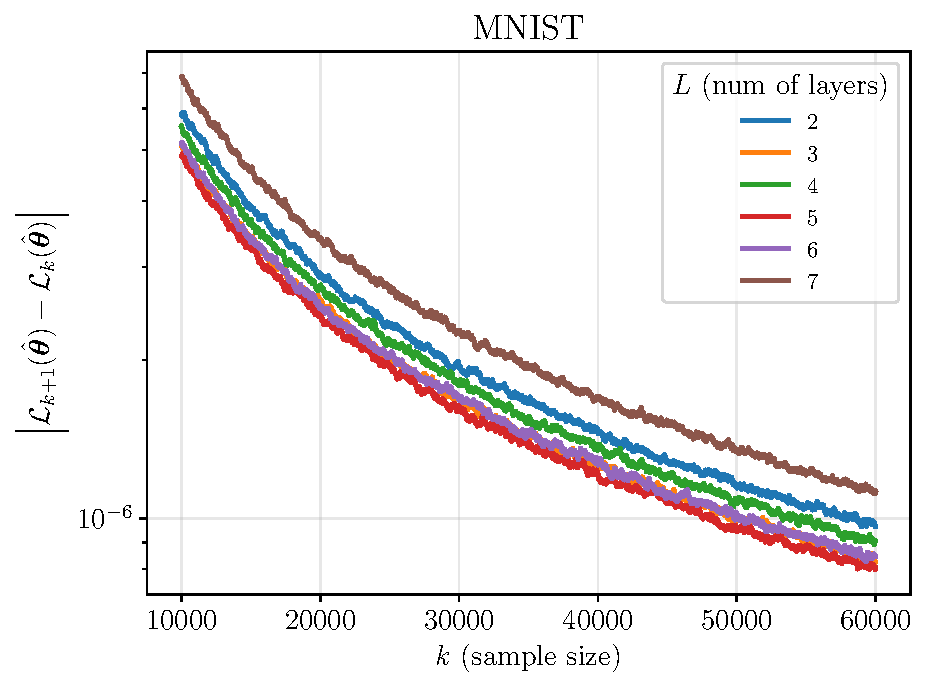
\includegraphics[width=\linewidth]{isp/figs/mnist_change_layers.pdf} 
    %\caption{Initial condition} 
    %\label{fig7:a} 
  \end{subfigure}%% 
  \begin{subfigure}[b]{0.5\linewidth}
    \centering
    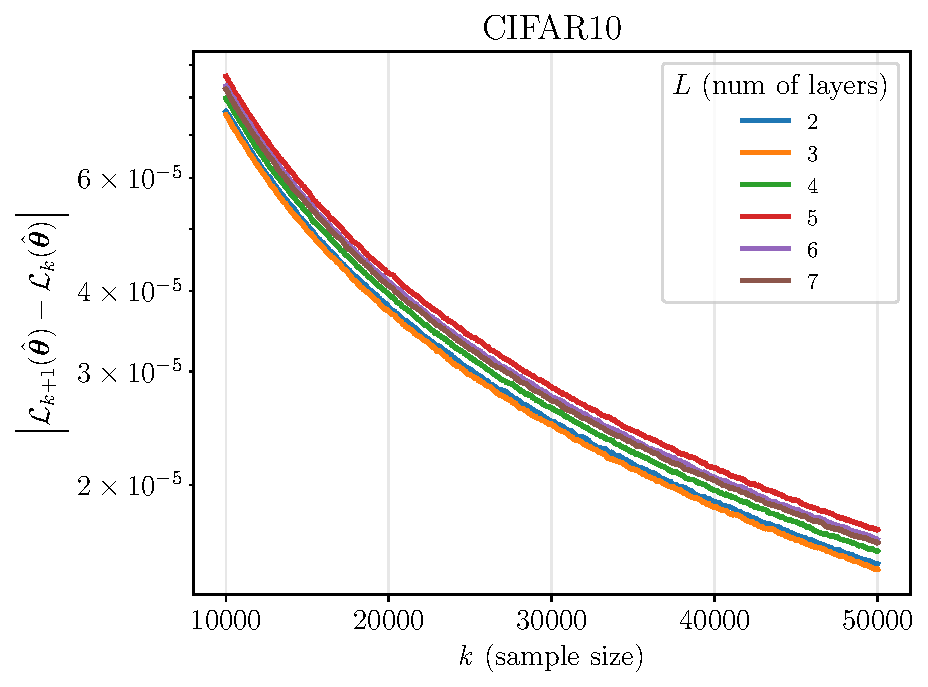
\includegraphics[width=\linewidth]{isp/figs/cifar10_change_layers.pdf} 
  \end{subfigure} 
  \caption{The variable number of hidden convolutional layers $L$ with fixed kernel size $k = 3$ and number of channels $C = 6$. Analysis of the resultant graphs reveals a non-monotonic relationship between the output values and the number of layers.}
   \label{fig:layers}
\end{figure}

\begin{figure}[ht]
  \begin{subfigure}[b]{0.5\linewidth}
    \centering
    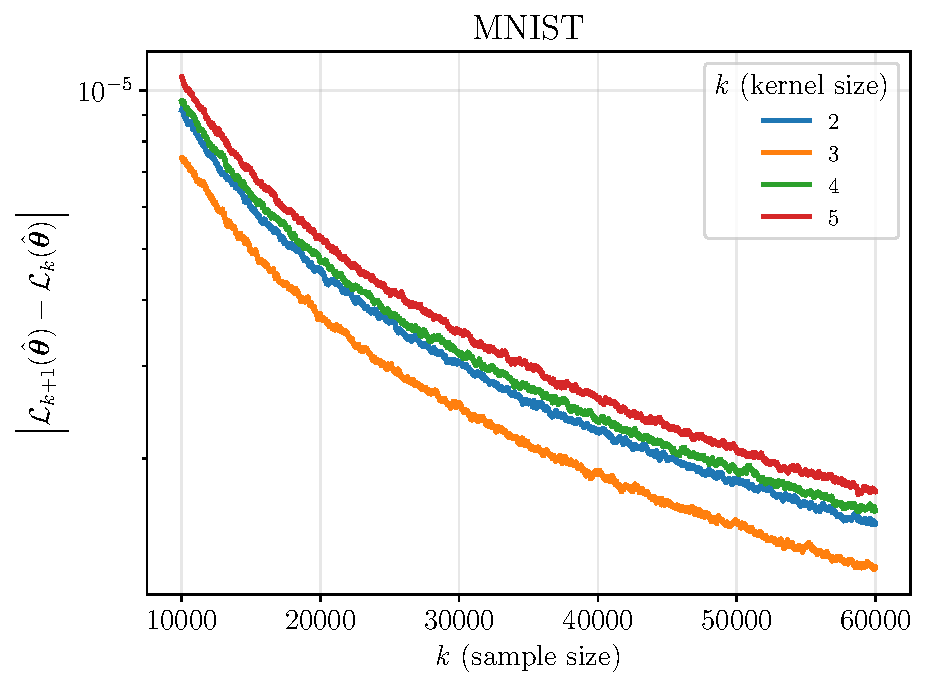
\includegraphics[width=\linewidth]{isp/figs/mnist_change_kers.pdf} 
    %\caption{Initial condition} 
    %\label{fig7:a} 
  \end{subfigure}%% 
  \begin{subfigure}[b]{0.5\linewidth}
    \centering
    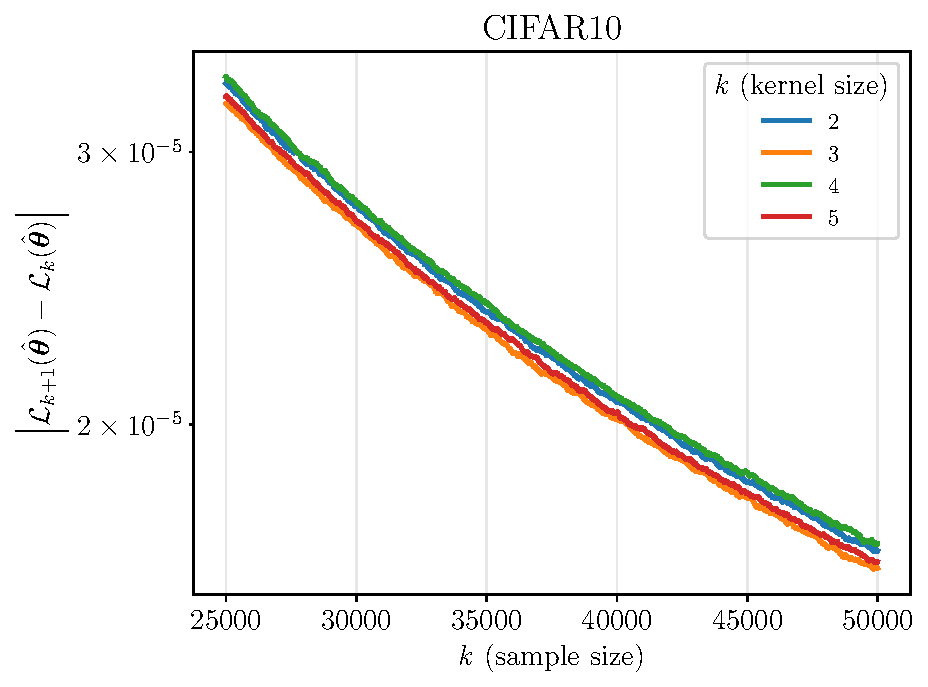
\includegraphics[width=\linewidth]{isp/figs/cifar10_change_kers.pdf} 
  \end{subfigure} 
  \caption{The variable the kernel size $k$ with fixed number of convolutional layers $L$ and number of channels $C = 6$. The data exhibit a non-monotonic relationship with respect to kernel size. }
   \label{fig:kernels}
\end{figure}

\begin{figure}[ht]
  \begin{subfigure}[b]{0.5\linewidth}
    \centering
    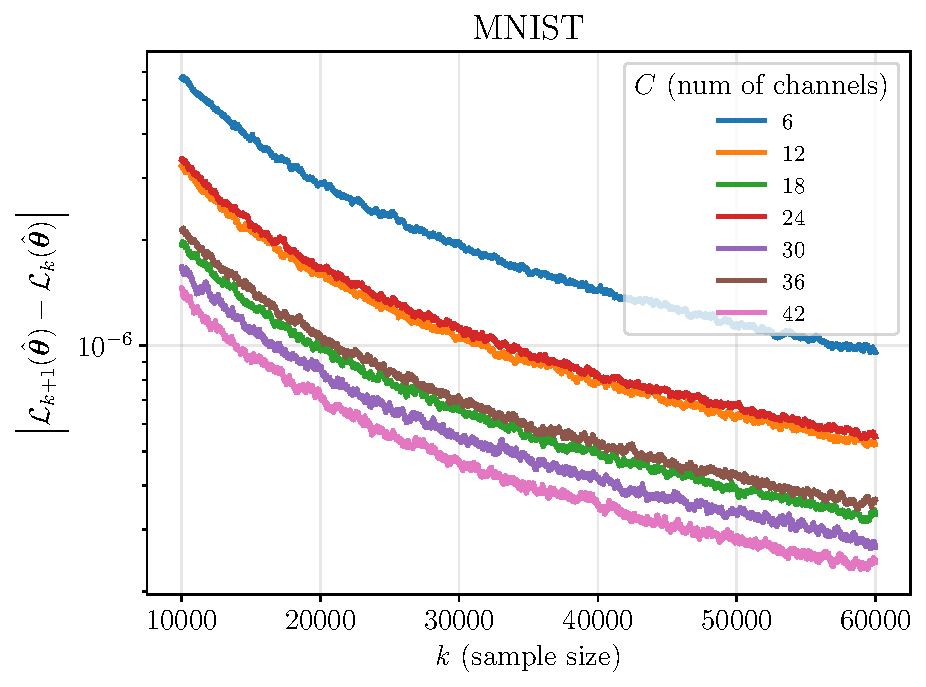
\includegraphics[width=\linewidth]{isp/figs/mnist_change_channels.pdf} 
    %\caption{Initial condition} 
    %\label{fig7:a} 
  \end{subfigure}%% 
  \begin{subfigure}[b]{0.5\linewidth}
    \centering
    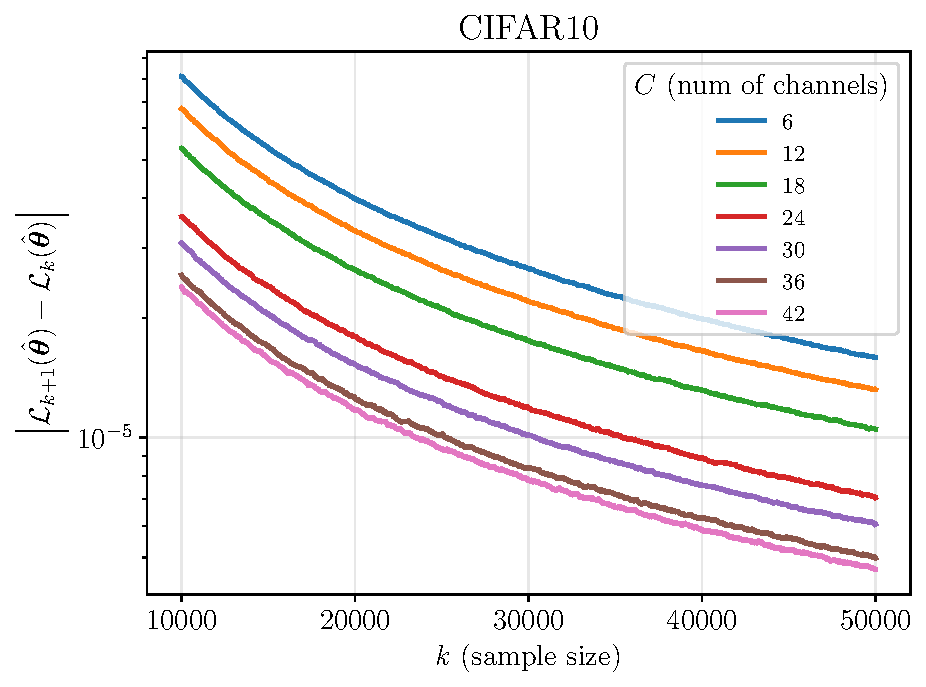
\includegraphics[width=\linewidth]{isp/figs/cifar10_change_channels.pdf} 
  \end{subfigure} 
  \caption{The variable channel num $C$ with fixed number of convolutional layers $L$ and kernel size $k=3$. The dependence of the value on the number of channels is monotonic.}
   \label{fig:channels}
\end{figure}

\begin{figure}[ht]
  \begin{subfigure}[b]{0.5\linewidth}
    \centering
    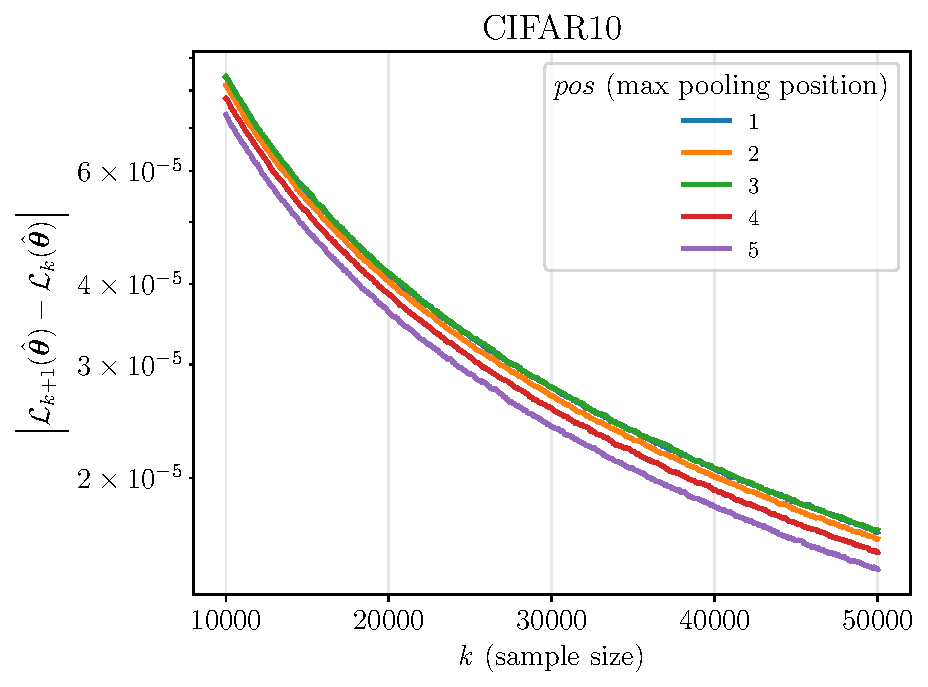
\includegraphics[width=\linewidth]{isp/figs/cifar10_change_maxpool_pos.pdf} 
    %\caption{Initial condition} 
    %\label{fig7:a} 
  \end{subfigure}%% 
  \begin{subfigure}[b]{0.5\linewidth}
    \centering
    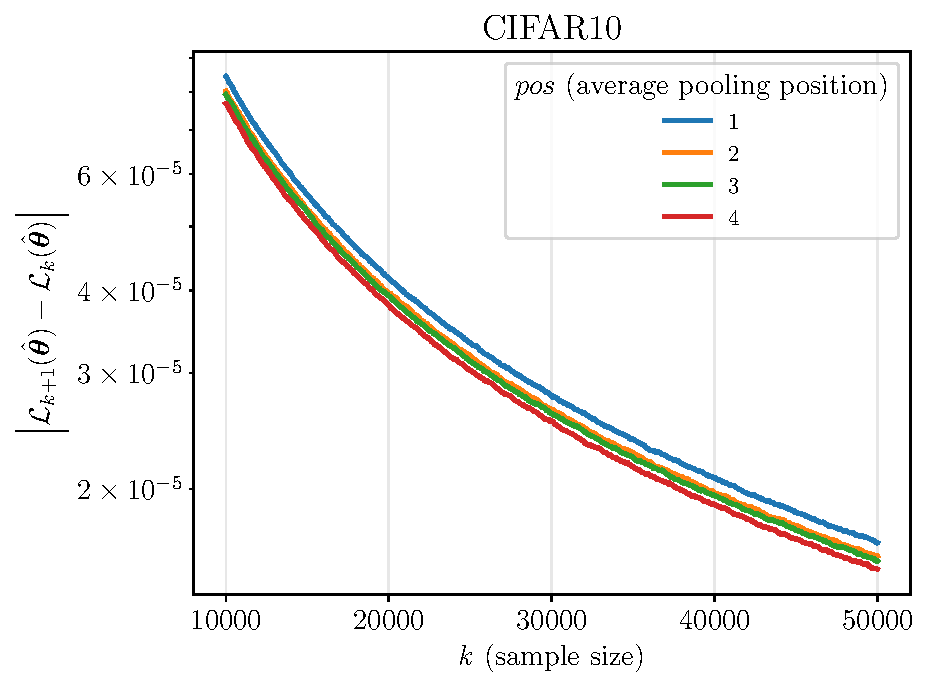
\includegraphics[width=\linewidth]{isp/figs/cifar10_change_avgpool_pos.pdf} 
  \end{subfigure} 
  \caption{The variable channels num $C$ with fixed number of convolutional layers $L$ and kernel size $k=3$. The graph shows a monotonic dependence of the value depending on the position of the pooling in the network.}
   \label{fig:pool_pos}
\end{figure}

\section{Discussion}\label{sec:disc}
As demonstrated by the graphs, the absolute difference between the average loss function values does not directly depend on kernel size or the number of network layers. However, it shows a monotonic relationship with layer size and pooling position. We suppose that this primarily indicates that the first part of Equation \eqref{eq:diff} has a more significant influence on this value. Consequently, it suggests that the loss function value at the optimum point is the predominant factor affecting this relationship. \\
It is noteworthy that the experiments employed relatively small networks, which means that increasing the number of parameters enhanced model quality, substantially influencing the results. In particular on the value of the loss function at optimum. \\
We have identified several potential solutions to this problem. First, we propose examining more complex network structures where increasing the parameter count would not have such a significant impact on our estimates. \\
Furthermore, it is evident that our estimation significantly exceeds realistic values and primarily serves as a theoretical construct rather than a practical measure. Primarily, the substantial overestimation can be attributed to the fact that the norm of matrix $\bT^{(p)}$ was evaluated through the product of norms (see proofs ~\ref{app:thm:1Dconv} or ~\ref{app:thm:2Dconv}), This approach, when applied to our specific case involving sparse matrices, inevitably leads to significantly overestimated results. The sparsity of the matrices in question exacerbates the discrepancy between the estimated and actual norms. \\
We posit that our research has potential applications in several areas, including exploring the functional landscape through analysis of the loss function's Hessian, developing techniques for determining appropriate sample sizes, and investigating the structural properties of neural network Hessian. These applications could contribute to a deeper understanding of neural network behavior.

\section{Conclusion}\label{sec:concl}
In this paper we proposed a method for estimating the Hessian norm, and also we have suggested a way to utilize this norm to estimate the convergence of the loss landscape. Using a second-order approximation of the loss function, our theoretical analysis suggests demonstrated how the convergence of the loss function landscape can depend on the norm of the Hessian, and also how the norm of the Hessian can depend on the parameters of the network. Our empirical results showed that the dependence of the absolute difference between the average loss function values has an ambiguous nature. We believe, that our results provide valuable insights into the local geometry of loss landscapes and properties of network hessian.

%%% BIBLIOGRAPHY %%%

\bibliographystyle{IEEEtran}
\bibliography{references}

%%% APPENDIX STARTED %%%
\appendices

\section{Proof of Lemma~\ref{lemma:hesstruct}}\label{app:lemma:hesstruct}
\begin{proof}
Output of our convolution is logits:
\[\bz = \f{x} = \bT^{(L+1)}\bLambda^{(L)}\bT^{(L)}....\bLambda^{(1)}\bT^{(1)}\bx.\]
We will work with derivative with respect to parameters
\begin{align*}
 \frac{\partial \bz}{\partial \bW^{(p)}} = \frac{\partial \bz}{\partial \bz^{(p)}}\frac{\partial \bz^{(p)}}{\partial \bT^{(p)}}\frac{\partial \bT^{(p)}}{\partial \bW^{(p)}} \;\text{ as a Jacobian of composition }
\end{align*}
Use $vec(\bB\bV\bA\T) = (\bA \otimes \bB)vec(\bV)$ with $\bA = \bI$ and get vectorized $\bz^{(p)}$ 
\[vec(\bz^{(p)}) = vec(\bT^{(p)}\bx^{(p-1)}) = (\bI \otimes \bx^{(p-1)})vec(\bT^{(p)}).\]
After one can see, that 
\[\frac{\partial \bz^{(p)}}{\partial \bT^{(p)}} = \bI \otimes \bx^{(p-1)\T}.\]
From $\bz = \bG^{(p)}\bz^{(p)}$ we achieve
\[\frac{\partial \bz}{\partial \bz^{(p)}} = \bG^{(p)}.\]
The definition of $\bQ^{(p)}$: \\
\[\frac{\partial\bT^{(p)}}{\partial\bW^{(p)}} = {\bQ}^{(p)}.\]
Using 
\[\bA_i \in \bbR^{m_i \times n_i} \text{ then } \bA_1 \otimes \bA_2 = (\bA_1 \otimes \bI_{m_2})(\bI_{m_1} \otimes \bA_2).\]
with $m_2 = 1$ we get
\[\bG^{(p)}\big(\bI \otimes \bx^{(p-1)\T}\big) = \big(\bG^{(p)} \otimes \bI_1\big)\big(\bI \otimes \bx^{(p-1)\T}\big) = \bG^{(p)} \otimes \bx^{(p)\T}.\]
we substitute the above statements into one formula and get
\[\frac{\partial \bz}{\partial \bW^{(p)}} = (\bG^{(p)} \otimes \bI_1)(\bI \otimes \bx^{(p-1)\T})\bQ^{(p)} = (\bG^{(p)} \otimes \bx^{(p)\T})\bQ^{(p)}.\]
As in \cite{singh2023hessianperspectivenatureconvolutional} consider the block $\bH_O^{(kl)}$:
\begin{align*}
& \bH_O^{(kl)} = J(\btheta)\T \bA J(\btheta) = \\
& = \bQ^{(k)\T}(\bG^{(k)\T} \otimes \bR^{(k-1)}\bx)A(\bG^{(l)} \otimes \bx\T\bR^{(l-1)\T})\bQ^{(l)}
\end{align*}
Then $\bH_O = \bQ^\bT\bF\bA\bF^\bT\bQ.$ \\
\end{proof}

\section{Proof of Lemma ~\ref{lemma:hessnorm}}\label{app:lemma:hessnorm}
\begin{proof}
Using the results of the previous Lemma ~\ref{lemma:hesstruct}, it is enough for us to evaluate the upper bound of the expression: $\norm{\bQ}^2\norm{\bF}^2\norm{\bA}$ \\
In the work \cite{kiselev2024unravelinghessiankeysmooth}, the norm of matrix $\bA$ was examined, and it was proven that: 
\[\norm{\bA} \leqslant \sqrt{2}.\] 
Norm of block-diagonal matrix is not greater than max of block's norm \\
\[\norm{\bQ}^2 \leqslant \max\limits_{i=1,\dots,L+1}\norm{\bQ^{(i)}}^2 \leqslant q^2.\] \\
Norm of matrix product is less or equal then product of norms:
\[\norm{\bG^{(p)}}^2 \leqslant \norm{\bT^{(p+1)}}^2 \dots\norm{\bT^{(L+1)}}^2 \leqslant w_{\bT}^{2(L - p + 1)}.\]
\[\norm{\bR^{(p-1)}}^2 \leqslant \norm{\bT^{(1)}}^2 \dots \norm{\bT^{(p-1)}}^2 \leqslant w_{\bT}^{2(p-1)}. \]
The spectral matrix norm of the Kronecker product is equal to their ordinary product norm. Spectral norm of vertical stacked matrices is less or equal then sum of norms of it's blocks
\begin{align*}
& \norm{\bF}^2 \leqslant \sum\limits_{p=1}^{L+1}\norm{\bG^{(p+1)\T}\otimes \bR^{(p-1)}\bx}^2 = \\ 
& = \sum\limits_{p=1}^{L+1}\norm{\bG^{(p)}}^2\norm{\bR^{(p-1)}\bx}^2.
\end{align*}
Substituting the obtained estimates into the $\norm{\bH_O}$ formula we get
\begin{align*}
& \norm{F}^2 \leqslant \norm{\bx}^2\sum\limits_{p=1}^{L+1}w_{\bT}^{2L} \leqslant \norm{\bx}^2(L+1)w_{\bT}^{2L}. \\
& \norm{\bH_O} \leqslant \norm{\bQ}^2 \norm{\bF}^2\norm{\bA} \leqslant \sqrt{2}\norm{\bx}^2q^2(L+1)w_{\bT}^{2L}.
\end{align*}

\end{proof}

\section{Proof of Theorem ~\ref{thm:1Dconv}}\label{app:thm:1Dconv}
\begin{proof}
It is clear that, based on the Lemma~\ref{lemma:hessnorm}, we need to proof only 2 statements:
\begin{align*}
 & \norm{\bT^{(p)}}^2 \leqslant C^2dkw^2, \\
 &\norm{\bQ^{(p)}}^2 \leqslant d^2.
\end{align*}
In \cite{singh2023hessianperspectivenatureconvolutional}, it is easy to see, that in $\bT^{(p)}$ every block of $C_lC_{l-1}$ has $d_{l-1}$ rows with kernel in the right position, which lead us to 
\[\norm{\bT^{(p)}}^2 \leqslant C^2dkw^2.\]

To prove the second inequality we again turn to \cite{singh2023hessianperspectivenatureconvolutional} and estimate the norm of vertically stacked matrices: \\
\[\frac{\partial \bT^{(l)}}{\partial \bW^{(l)}} =: \bQ^{(l)} = \bI_{C_l} \otimes
    \begin{pmatrix}
        \bI_{C_{l-1}} \otimes (\pi_R^0\bI_{d_{l-1} \times k_l}) \\
        \vdots \\
        \bI_{C_{l-1}} \otimes (\pi_R^{d_{l-1} - k_l}\bI_{d_{l-1} \times k_l})
    \end{pmatrix}.
\]
\begin{align*}
& \norm{\bQ^{(l)}} \leqslant \sum\limits_{i=0}^{d_{l-1} - k_l}\norm{\pi_R^i\bI_{d_{l-1} \times k_l}} \leqslant \sum\limits_{i=1}^{d_{l-1} - k_l}\norm{\pi_R} = \\
&= \sum\limits_{i=0}^{d_{l-1}-k_l} 1 = d_{l-1} - k_l + 1 = d_l \leqslant d_1 = d. \\
\end{align*}
\end{proof}

\section{Proof of Theorem ~\ref{thm:2Dconv}}\label{app:thm:2Dconv}
\begin{proof}
from the description ~\ref{sec:2d-conv} of the matrix $\bT^{(p)}$ one can see, that
\[\norm{\bT^{(p)}_{i, *}}^2 = \sum\limits_{c, k, l}^{C_{p-1}, k_p^1, k_p^2}|\bW^{(p)}_{c, c_2, k, l}|^2.\] \\
And as an obvious consequence \\
\begin{equation}\label{eq:estim_toep_2d}
\norm{\bT^{(p)}}_F^2 = \sum\limits_{c_1, i, k, l}^{C_{p-1}, C_pn_pm_p, k_p^1, k_p^2}\big(\bW^{(p)}_{c_1, c_2(i), k, l}\big)^2.
\end{equation}
Here we assume a simple correspondence between the output channel $c_2$ and the $\bT^{(p)}$ line $i$.

By analogy with the proof ~\ref{app:thm:1Dconv}, using ~\ref{lemma:hessnorm} we need to proof 2 statements: \\
\[\norm{\bT^{(p)}} \leqslant C^2k^2w^2mn.\]
\[\norm{\bQ^{(p)}} \leqslant C^2k^2mn.\]
Initially, the norm of $\bT^{(p)}$ is estimated:
\[\norm{\bT^{(p)}}^2 \leqslant \norm{\bT^{(p)}}_F^2 \leqslant |_{\text{use } \eqref{eq:estim_toep_2d}}| \leqslant \sum\limits_{i} Ck^2w^2 \leqslant C^2k^2w^2mn.\] \\
Next, we will estimate norm of the layer derivative with respect to the parameters.
\[\norm{\bQ^{(p)}} = \norm{\frac{\partial \bT^{(p)}}{\partial \bW^{(p)}}}.\]
As stated earlier the row of $\bT^{(p)}$ - it is exactly $vec_r(\bW^{(p)}_{*, i, *, *})$ arranged in the correct order.
Then the norm of the row is: \\
$\frac{\partial \bT^{(p)}_{(i, j)}}{\partial \bW^{(p)}_{c_1, c_2, k_1, k_2}} \neq 0 \iff$ the indices are selected in such a way, that $T^{(p)}_i$ corresponds $c_2$ and at the same time $\bT^{(p)}_{i, j}$ corresponds $c_1, k_1, k_2$ and this correspondence depends on the specific matrix $\bT^{(p)}$, but it is obvious, that one $i$ corresponds to only one $c_2$, because every row participates in the formation of only one element of one channel. Since only $\bW^{(p)}_{*, c_2, *, *}$ participates in the formation of one line $\bT^{(p)}_{i, *}$, we can fixed $i$ and corresponding $c_2$, and also at the same time we know that, for every $c_1, k_1, k_2$, there are only one column $j$: $\bT^{(p)}_{i, j} = \bW^{(p)}_{c_1, c_2, k_1, k_2}$:
\begin{align*}
& \sum\limits_{j,c_1, k_1, k_2}\bigg(\frac{\partial \bT^{(p)}_{i, j}}{\partial\bW^{(p)}_{c_1, c_2, k_1, k_2}}\bigg)^2 = \\
& \sum\limits_{c_1, k_1, k_2}\sum\limits_{j}\bigg(\frac{\partial \bT^{(p)}_{i, j}}{\partial\bW^{(p)}_{c_1, c_2, k_1, k_2}}\bigg)^2 = \\
& = |_{\text{in the inner sum there is only one non-zero term}}| = \\
& = \sum\limits_{c_1, k_1, k_2}1 = C_{p-1}k_p^1k_p^2 \leqslant Ck^2.
\end{align*}
Consider the Frobenius norm as the upper bound of the spectral norm:
\begin{align*}
& \norm{\bQ}^2 \leqslant \norm{\bQ}^2_F = \sum\limits_{i, j, c_1, c_2, k_1, k_2}\bigg(\frac{\partial \bT^{(p)}_{i,j}}{\partial \bW^{(p)}_{c_1, c_2, k_1, k_2}}\bigg)^2 = \\
& = \sum\limits_{i, c_2}\sum\limits_{j, c_1, k_1, k_2}\bigg(\frac{\partial \bT^{(p)}_{i,j}}{\partial \bW^{(p)}_{c_1, c_2, k_1, k_2}}\bigg)^2 = \\
& = |_{\text{estimated the internal sum earlier and only under appropriate $i$ and $c_2$}}| \leqslant \\
& \leqslant \sum\limits_{i}Ck^2 = CmnCk^2 \leqslant C^2k^2mn.
\end{align*}
\end{proof}

\section{Proof of the Lemma ~\ref{lemma:maxpool}}\label{app:lemma:maxpool}
\begin{proof}
Let's use the notation $\bM^{(l)}$ for our 2D-Max-Pool layer \\
Like for convolutions, we can describe every row $\bM^{(l)}$: \\
Before starting, there some properties of $\bM$, that which will be used: At first, that the row $\bM_{i*}$ corresponds to specific pooling window(to elements covered by window), and, as the second one, is that column $\bM_{*j}$ corresponds to elements are multiplied by $j$'th element of input. \\
Since every window covers only one element and 2 different windows do not intersect, then there are only one element in every row, thus
\[\norm{\bM^{(l)}} = \sqrt{\lambda_{max}({\bM^{(l)\T} \bM^{(l)}})} = 1,\] \\
because $(\bM^{(l)}_{*, i}, \bM^{(l)}_{*, j}) \neq 0 \iff (\bM^{(l)}_{*, i}, \bM^{(l)}_{*, j}) = 1 \iff i = j $ and i'th element is max in appropriate window. For simplicity, we assume that $\bM^{(l)}$ reduces both dimentions ${k_{\mathrm{pool}}}$ times Similar to the ~\ref{app:thm:2Dconv} we estimate $\bG^{(p)}$ and $\bR^{(p-1)}$ component, however, in accordance with the new layer
\begin{align*}
& \norm{\bG^{(p)}}\norm{\bR^{(p-1)}} \leqslant \frac{\prod\limits_{i=1}^{L+1}\norm{T^{(i)}}}{\norm{T^{(p)}}} \leqslant \\
& (C^2k^2w^2mn)^{2L}\bigg(\frac{1}{k_{\mathrm{pool}}^2}\bigg)^{L - l + 2 - I\{p-1 \leqslant l\}} \leqslant \\
& (C^2k^2w^2mn)^{2L}\bigg(\frac{1}{k_{\mathrm{pool}}^2}\bigg)^{L - l + 2}
.
\end{align*}
Then we have
\begin{align*}
& \norm{\bF}^2 \leqslant \norm{\bx}^2(L+1)(k^2C^2w^2mn)^{(L)}\big(\frac{1}{k_{\mathrm{pool}}^2}\big)^{L - l + 2}, \\
& \norm{\bH_O} \leqslant \sqrt{2}\norm{\bx^2}q^2\big(\frac{1}{k_{\mathrm{pool}}^2}\big)^{L-l+2}(L+1)(k^2C^2w^2mn)^{L},
\end{align*}
where $q^2 = mnC^2k^2.$
\end{proof}

\section{Proof of the Lemma ~\ref{lemma:avgpool}}\label{app:lemma:avgpool}
\begin{proof}
    We use the notation $\bA^{(l)}$ for our 2D-Avg-Pool layer \\
    One can see, that
    \[(\bA_{*, i}, \bA_{*,j}) = \frac{1}{k_{\mathrm{pool}}^4}I\{\text{i, j corresponds to the same window}.\}\] \\
    To achieve this, we can see into formula: \\
    $(\bA_{*j}, \bA_{*i}) = \sum\limits_{k}\bA_{ki}\bA_{kj} = \sum\limits_{k:\bA_{ki} \neq 0, \bA_{kj} \neq 0}\frac{1}{k_{\mathrm{pool}}^4}$. \\
    After this, applying elementary transformations over rows and columns, we reduce matrix $\bA^{(p)\T}\bA^{(p)}$ to a block-diagonal form, where blocks correspons indexes in the same avg-pool window. Each block of $\bA^{(p)\T}\bA^{(p)}$ is $\bB_i = \frac{1}{k_{\mathrm{pool}}^2}\mathbf{11}\T$, where $\mathbf{1} = \mathbf{1}_{k_{\mathrm{pool}}^2} \in \bbR^{k_{\bA}^2}$ - vector of ones, and it's norm $\norm{\bB_i} = \frac{1}{k_{\mathrm{pool}}^2}\norm{\mathbf{11\T}} = \frac{1}{k_{\mathrm{pool}}}$ \\
    Norm of block-diagonal matrix (and the norm of a matrix that can be reduced to this form) is max of norms: \\
    $\norm{\bA^{(p)}} = \max\limits_{i}\norm{\bB_{i}} = \frac{1}{k_{\mathrm{pool}}}$, \\
    because of $\norm{\bA^{(p)}} \leqslant 1$, we can use completely reuse the calculations of the previous proof and have the same result.
\end{proof}

\section{Proof of Lemma ~\ref{lemma:fc-head}}\label{app:lemma:fc-head}
\begin{proof}
As in previous proofs we need to estimate $\norm{\bG^{(p)}}^2\norm{\bR^{(p-1)}}^2$. \\
We know, that $\norm{T^{(L+1+p)}}^2 \leqslant (h^2\tilde{w}^2)\; \forall p = 1, \dots, P$
Then, we can estimate
\[\norm{\bG^{(p)}}^2\norm{\bR^{(p-1)}}^2 \leqslant (h^2\tilde{w}^2)^{P}(k^2C^2w^2mn)^L,\] for $p \leqslant L+1$ and \\
\[\norm{\bG^{(p)}}^2\norm{\bR^{(p-1)}}^2 \leqslant (h^2\tilde{w}^2)^{P-1}(k^2C^2w^2mn)^{L+1},\] 
for $p = L+2 \dots L+P+1$. \\
Or in one entry: \\
\[\norm{\bG^{(p)}}^2\norm{\bR^{(p-1)}}^2 \leqslant (h^2\tilde{w}^2)^{P-I_{\{p > L+1\}}}(k^2C^2w^2mn)^{L + I_{\{p > L+1\}}}.\] \\
Then we have: \\
\begin{align*}
& \norm{F}^2 \leqslant \sum\limits_{p=1}^{L+P+1}\norm{\bG^{(p)}}^2\norm{\bR^{(p-1)}}^2\norm{x}^2 \leqslant \\
& (h^2\tilde{w}^2)^P(k^2C^2w^2mn)^{L}\big(L+1 + P\frac{h^2\tilde{w}^2}{k^2C^2w^2mn}\big).
\end{align*}
And applying this result to the Hessian \\
\begin{align*}
& \norm{\bH_{O}} \leqslant \sqrt{2}W_{x}q^2(h^2\tilde{w}^2)^P(k^2C^2w^2mn)^L\times \\
& \times \big(L + 1 + P\frac{h^2\tilde{w}^2}{k^2C^2w^2mn}\big).
\end{align*}

\end{proof}

\end{document}
